\newpage
\section{Wissenschaftlicher Teil}

\subsection{Analyse des Forschungsstandes}

\subsection{Erläuterung des Anwendungsfalles}
Der Anwendungsfall beschreibt Gastronomen, die Unterstützung bei der Generierung von Social Media Inhalten benötigen, um die Attraktivität, die Aufmerksamkeit und den Umsatz ihres Lokals zu steigern.
Dabei wird eine Lösung entwickelt, welche Front-end-basierend den Gastronomen zu einem Social Media-Post führt.
Die Lösung setzt dabei auf Künstliche Intelligenz in Form von Large Language Modellen, um Bilder und kreative Beiträge zu generieren.
Dabei kann der Gastronom selbst, mit Unterstützung, Einfluss auf die generierten Inhalte nehmen.
Allesamt sollen die generierten Inhalte, basierend auf der Frontendführung, zu einem Social Media Post führen, welcher direkt aus dem Frontend getätigt werden kann.
Neben der Generierung der Social Media Posts soll der Gastronom über das Frontend die Möglichkeit haben einen Kalender einzusehen, in welchem aktuelle Social Media Kampagnen laufen und gegebenenfalls welche planen können.
Damit eine Lösung adäquat und tragend entwickelt werden kann, bedarf es erst einer Markt- und Wettbewerbsanalyse, die strategische Auswahl einer Social Media Plattform und ein Konzept zur Monetarisierung der entwickelten Lösung.
Hierbei soll sich der erste Anwendungsfall vorerst auf nur eine Social Media Plattform konzentrieren, da sich alle Social Media Plattformen heterogen zueinander verhalten.

\subsection{Markt- und Wettbewerbsanalyse}
Die Markt- und Wettbewerbsanalyse ist ein Vorgehen, welches eingesetzt wird, um eine Übersicht über die Möglichkeiten am Markt und die potenziellen Wettbewerber zu erlangen.
Dabei bietet der Markt, bezogen auf den Anwendungsfall, vielversprechende Möglichkeiten im Einsatz von Generativer Künstlicher Intelligenz im Social Media Marketing Bereich bei Kleinen und Mittelständischen Unternehmen.
So geht aus einer Datenerhebung durch Statista hervor, dass das Wachstum von KI-basierenden Lösungen im Marketingbereich groß ist und bis zum Jahr 2028 einen Umsatz von bis zu 107.5Mrd. USD erreichen kann.\footcite{statista_ai_marketing_europe}

Ebenfalls zeigt eine Studie von McKinsey, dass der Einsatz von Technologien, wie Generative Künstliche Intelligenz, das Potenzial haben eine erhebliche Steigerung der Produktivität haben.\footcite{mckinsey_genai_marketing}

In der Gastronomiebranche wird die Wichtigkeit und die potenzielle Chance von Social Media Marketing besonders deutlich dadurch, dass ca. 37 Prozent\footcite{apicbase_gastro_fakten} der Gäste die Social Media Seiten der Gastronomien besuchen, um über diese Informationen zu erlangen und generell informieren sich ca. 84 Prozent\footcite{g_wie_gastro_trends_2024} der Gäste über ein Lokal erst online.
Ebenfalls lässt sich sagen, dass laut einer Erhebung von Statista die Interaktion sich zwischen Gastronomen und Gästen geändert hat, seitdem Social Media Plattformen populärer wurden.\footcite{statista_social_media_gastgewerbe}

Bei diesem potenziellen Markt gibt es ebenfalls schon einige Wettbewerber, die Social Media Marketing mithilfe von Generativer Künstlicher Intelligenz betreiben.
Drei direkte Wettbewerber sind Killian, MARA und Jasper.ai.

Killian ist eine speziell auf die Hotel- und Restaurantbranche ausgerichtete Lösung, die diverse Funktionalitäten anbietet, wie z. B. Bewertungsmanagement, Content Manage-ment, E-Mail-Marketing, Public Realtions, und Social Media.\footcite{kilian_ai_produkt}
Dabei setzt Killian auf Generative Künstliche Intelligenz und setzt Modelle, wie u. a. GPT4, hierfür ein.
Klare Vorteile dieser Lösung sind die Umfänglichkeit und der Fokus auf die Gastronomie- und Hotelbranche im Einsatz von Generativer Künstlicher Intelligenz.
Nachteile, die sich hervortun, sind das Bezahlmodell, in Form einer 14-Tägien Testversion mit anschließendem Zwang zum Kauf einer Premiumvariante\footcite{kilian_ai_preise} und keiner End-to-End-Funktionalität, im Sinne von keiner Möglichkeit direkt aus der Applikation auf Social Media etwas zu publizieren.\footcite{kilian_ai_funktionen}
Dementsprechend ist die Spezialisierung auf Social-Media nicht vollständig ausgereift bei der Lösung Killian.

MARA positioniert sich als Bewertungsmanagementlösung, unter Einsatz von Generativer Künstlicher Intelligenz, als weiterer Wettbewerber.
Dabei liegt der Fokus dieser Lösung primär auf die Bearbeitung von Bewertungen, wie z. B. Google Bewertungen, oder auf Social Media Plattformen, jedoch nicht auf die Generation von Branchenspezifi-scher Inhalte, wie in dem Fall der Gastronomiebranche.
MARA setzt auch auf keine Art der Bildgenerierung.
Damit ist diese Lösung kein direkter Konkurrent und könnte synergierend genutzt werden.\footcite{mara_solutions_features}

Der dritte Wettbewerber, Jasper.ai, setzt auf ein generisches KI-Tool für die Generierung von Content-Marketing.
Von der Generierung von Texten bis hin zur Generierung von Bildern ist mit diesem Tool alles möglich.
Jedoch ist Jasper.ai nicht branchenspezifisch.\footcite{jasper_ai_product_marketers}

Ein Nachteil an allen drei direkten Wettbewerbern ist die Benutzbarkeit der Lösungen.
Der Einsatz der Lösungen erfordert eine gewisse IT-Affinität, welche bei Gastronomen nicht zwangsläufig vorausgesetzt werden sollte, da ihre Stärken in den gastronomischen Bereichen liegen.

Indirekte Wettbewerber, die in einem Vergleich nicht fehlen dürfen, sind einerseits Werbeagenturen, die sich u. a. um den Social Media Auftritt kümmern. Diese liefern maßgeschneiderte Lösungen, sind aber in aller Regel teurer und weisen längere Produk-tionszeiten der Inhalte auf, als maschinell generiete Inhalte.
Andrerseits gibt es auch Freelancer, die sich um den Social Media Auftritt von Gastronomen kümmern könnten.
Diese könnten jedoch den Nachteil von einer inkonsistenten Qualität der Inhalte auf-weisen, wie z. B. qualitativ minderwertige Beiträge oder Unzuverlässigkeit.
Der Vorteil könnte die Kosteneffizienz sein und die Flexibilität.

\subsection{Kundenanalyse}
Ein Aspekt in der Betrachtung des zukünftigen Kunden, ist die Festlegung des stereotypischen Kunden, der für diese Applikation in Frage kommt.
Für die Festlegung wird in erster Linie die Zielgruppe definiert und die Erwartungen der Kunden, an diese Applikation, evaluiert.

Die primäre Zielgruppe sind kleine und mittelständische Gastronomiebetriebe, da diese die Hauptkunden der DISH-Consulting GmBH sind.
KMU-Gastronomiebetriebe können exemplarisch kleine lokale Pizzalieferdienste bis hin zu mittelgroßen Restaurants sein.
Diese haben oftmals die Problematik, dass keine notwendigen Kompetenzen im Betrieb vorhanden sind, um ein ordentliches Marketing-Konzept zu betreiben, da es oftmals zu teuer ist.\footcite{restroworks2024}
Unter ein ordentliches Marketing-Konzept würde ebenfalls auch der Einsatz von Social-Media-Maßnahmen fallen.

Dementsprechend könnten Erwartungen von zukünftigen Kunden dieser Applikation sein, dass exakt diese Problematiken kosteneffizient aufgegriffen werden.
Genauer gesagt antizipieren sich die Erwartungen dahingehend, dass hochwertiger Social-Media-Content generiert werden soll, der als Teil einer Marketingmaßnahme die Bekanntheit des Gastronomiebetriebs steigern soll.
Aus einer höheren Bekanntheit des Betriebes würden sich die Betreiber höhere Umsätze, wegen mehr Bestellungen oder Besuche, erhoffen.
Eine weitere Erwartung an die Generierung des hochwertigen individuellen Social-Media-Contents dürfte die einfache Bedienung einer solchen Applikation sein, da die wenigstens Gastronomen IT-Affin sind.

All diese Erwartungen lassen sich übergeordnet in die Sammelbegriffe Umsatzoptimierung, Zeiteffizienz, Kostenersparnis und Prozessoptimierung klassifizieren.

\subsection{SWOT-Analyse}
Die SWOT-Analyse dieser Lösung soll die Stärken, Schwächen, Chancen, als auch Risi-ken aufzeigen, um eine Übersicht der Möglichkeiten zu generieren.
Eine Stärke dieses Tools ist vor allem die Branchenspezialisierung, welche eine maßgeschneiderte Lösung für Gastronomen bietet.
Eine weitere Stärke bildet die End-to-End-Lösung, welche erlaubt, dass Gastronomen direkt aus dem Tool Content generieren und veröffentlichen können.
Die dritte und wichtigste Stärke dieser Lösung ist die Benutzerfreundlichkeit, welche jegliche Einstiegshürden für technisch weniger versierte Nutzer reduziert.

Die schwerwiegendsten Schwächen dieses Tools sind zum einem die technologische Abhängigkeit von der Qualität und Weiterentwicklung der Large Language Modelle und zum anderen die etablierte Konkurrenz, welche bereits eine starke Marktpräsenz haben.
Die Chancen, die durch den Einsatz dieses Tools entstehen, sind zum einem die wach-sende Nachfrage nach Automatisierung, durch steigende Akzeptanz von KI-Tools in der Gastronomie.
Zum anderen das Potenzial zur Expansion auf weitere Branchen, wie z. B. die Hotellerie und zuletzt die Möglichkeit einzigartige Inhalte zu generieren, die individuell auf den Kunden zugeschnitten sind.

Mögliche Risiken durch den Einsatz dieses Tools sind Datenschutzbedenken.
Kunden, die das Tool einsetzen könnten, könnten sich zurückhalten aufgrund der Erhebung von sensiblen Daten.
Ein anderes Risiko, welches besteht, sind die schnellen Innovationen am Markt.
Der Markt, in der Gastronomie und KI, entwickelt sich stetig weiter, sodass ggf. schnelle Anpassungen der Lösung erforderlich sind.

\subsection{Strategische Auswahl der Social Media Plattformen}
Ergänzend zur Markt- und Wettbewerbsanalyse bedarf es ebenfalls an einer strategischen Auswahl einer geeigneten Social Media Plattform.
In einer ersten Iteration der Entwicklung einer GenAI Social Media Kampagnen Lösung ist es sinnvoll sich auf eine Plattform zu begrenzen, da die zur Verfügung stehenden Social Media Plattformen zwar im Kern dasselbe bezwecken, jedoch jede Plattform eigen für sich funktioniert.
Zur Auswahl stehen laut dem „Digital 2024 Global Overview Report“ von Hootsuite eine Vielzahl an Social Media Plattformen.
Gemessen an den aktiven Benutzern auf den Plattformen bilden die fünft meist benutzten Social Media Plattformen Facebook (ca. 3.05Mrd.), YouTube (ca. 2.49Mrd.), WhatsApp (ca. 2.00Mrd.), Instagram (2.00Mrd.) und TikTok (ca. 1.56Mrd.).\footcite{hootsuite_digital_2024_page_232}
Zu betrachten ist bei dieser Aufzählung, dass das Unternehmen Meta hier drei von fünf Plattformen (Facebook, WhatsApp und Instagram) betreibt.
Die Social Media Plattformen YouTube und TikTok sind Plattformen, die primär Videos in Form von Lang- und Kurzformaten anbieten.
Das bedeutet, dass sämtliche Beiträge, die dort durch Benutzer erstellt werden, ausschließlich Videobeiträge sind.
Die Plattform WhatsApp ist in erster Linie ein Messenger-Dienst, der für Privatnachrichten und Anrufe zwischen mehreren Personen genutzt werden kann.
Dies funktioniert jedoch nur dann, wenn die Telefonnummern den Personen bekannt sind, im Gegensatz zu den anderen Social Media Plattformen, die auf Nutzernamen setzen.
Instagram, als auch Facebook setzen auf eine Art Plattform, bei dem jeder Benutzer öffentliche, als auch private Bild-, Text-, Videobeiträge generieren kann, die entweder der gesamten Nutzerschaft der Plattform angezeigt werden könnten oder nur den befreundeten Be-nutzern auf der Freundesliste.
Ebenfalls können sich Benutzer auf diesen beiden Platt-formen per private Nachrichten kontaktieren, ähnlich wie bei WhatsApp.

Zur Auswahl einer geeigneten Social Media Plattform, die sich für einen ersten Prototypen eignet, wird auf die beliebteste der fünf aufgezählten Social Media Plattformen gesetzt – Instagram.
Aus dem „Digital 2024 Global Overview Report“ von Hootsuite geht hervor, dass Instagram, trotz der geringeren Nutzerzahl zu Facebook, WhatsApp und YouTube, dennoch die beliebteste bei Nutzern zwischen dem Alter 16 und 64 ist, wie aus dem Report hervorgeht.\footcite{hootsuite_digital_2024_page_236}
Ebenfalls geht aus diesem Report hervor, dass ca. 63 Prozent der Nutzer der Plattform Instagram im Alter zwischen 16 und 64, diese Plattform nutzen, um Unternehmen zu suchen und investigieren.\footcite{hootsuite_digital_2024_page_250}
Dementsprechend liegt die Wahl der ersten anzubindenden Social Media Plattform für den Prototypen bei Instagram.

\subsection{Strategie zur Monetarisierung des Anwendungsfalles}
Zu einer vollständigen Betrachtung des Anwendungsfalles gehört ebenfalls auch die Monetarisierung der Lösung.
Im Fokus steht zum einem die frontendgeführte Generierung von Social Media Posts und der Kalender, welcher zur Übersicht und Planung weiter Social Media Posts genutzt werden kann.
Ein Ansatz dieses Produkt zu vermarkten wäre das sogenannte Freemium-Modell.
Dieses beschreibt ein Vermarktungsmodell, bei dem eine kostenlose Basisvariante des Produktes zur Verfügung steht und weitere, bzw. vollwertige Funktionalitäten bei Erwerb der Premiumvariante freigeschaltet werden.
Im konkreten Anwendungsfall würde das bedeuten, dass der Kunde, der den entwickelten AI basierenden Social Media Manager nutzen möchte pro Monat bis zu fünf Beiträge sich kostenlos generieren lassen könnte und jede weitere Benutzung würde Geld kosten.
Ebenfalls würde erst die Funktionalität des Kalenders erst gegen Entgelt zur Verfügung stehen.
Damit würde sich die entwickelte Lösung durch seine Abonnements tragen.
Neben der offensichtlichen Monetarisierung der entwickelten Lösung, könnte man durch Einwilligungserklärungen der Gastronomen deren eingegebenen Daten verarbeiten, sodass ein weiteres Konzept der Monetarisierung entsteht.
Die erhobenen Daten, die bspw. durch die Kalenderfunktionalitäten entstehen, wie „Wann plane ich einen Beitrag?“, oder „Wie viele Kampagnen laufen aktuell?“, könnten wertvolle Einblicke von Gastronomen generieren, die für entweder an Interessenten verkauft werden könnten, oder es werden weitere Machine Learning-basierende Anwendungsfälle entwickelt, wie z.B. „Wann ist der beste Zeitpunkt für eine Kampagne?“ und monetarisiert diesen wieder.
Genauso ist die Erhebung der Prompts ein wichtiger Datenerhebungsaspekt zur Monetarisierung und konzeptioniert weiterer Funktionalitäten dieses Anwendungsfalles.


\subsection{Evaluation einzusetzender Technologien}

\subsection{Evaluation und Auswahl generativer Machine Learning Modelle}
Die in Kapitel XYZ genannten Eigenschaften beschreiben die wichtigsten Charakteristiken von Social Media Content, um die Aufmerksamkeit und Interaktionsrate von Social Media Nutzern zu maximieren und somit potenzielle Leads zu generieren und zu einer Kaufentscheidung für ein beworbenes Produkt zu bringen.
Hierbei ist zu beachten, dass der Content ideal auf die jeweilige Social Media Plattform abgestimmt ist und die Zielgruppe emotional anspricht, damit sich dieser besser in Erinnerung bleibnt.
Zudem sollte der Content eine klare und konsistente Botschaft transportieren.

Zudem sollten veröffentliche Inhalte einen Hochwertigen Eindruck vermitteln und sowohl farblich als auch typografisch mit der Markenidentität übereinstimmen.
Eine zentrale Aufgabe im Bereich des Social Media Marketings ist somit die Erstellung und veröffentlichung von hochwertigem, zielgruppen gerichteten und aussagekräftigen Content, der Zielgruppen zu einer Kaufentscheidung bringt, oder im allgemeinen den Wiedererkennungswert eines bestimmten Produktes oder einer gesamten Marke  steigert.

Die generierung von Social Media Content ohne den Einsatz von generativen Machine Learning Modellen erfordert umfangreiche Ressourcen, um ein qualitativ hochwertiges Ergebnis zu erzielen.
Um hochwertige Social Media Werbeinhalte zu erzeugen werden diverse Kompetenzen in den Bereichen, Kreativität, Marketing, Design, Fotografie und Ton benötigt.
Aus den daraus resultierenden Kosten zeichnet sich ein Trend im Einsatz von generativen Machine Learning Modellen ab. (Hier paar Facts).

Diese Entwicklung hat dazu geführt, dass heutige state-of-the-art KI Modelle dazu Fähig sind, Social Media Content jeglicher Art, egal ob in Bild-, Text-, oder Videoform zu erzeugen, welcher sich ohne Weiteres nicht von menschlich generierten Content unterscheiden lässt und den Eindruck von hochwertig generierten Werbeinhalten vermittelt.
Auf eine Vielzahl dieser äußerst leistungsfähigen Modelle kann über das Internet kostenlos zugegriffen werden.
Machine Learning Plattformen wie Hugging Face bieten die möglichkeit, vortrainierte Machine Learning Modelle aus verschiedensten Kategorie, wie beispielsweise text-to-image, text-to-text, text-to-voice und viele Weitere, kostenlos herunterzuladen und auf eigenen Hardware Ressourcen zu betreiben und zu verwenden.
Die Auswahl des zu verwendenden Machine Learning Models ist neben der Erschaffung eines optimalen prompts zur Nutzung des Modells von zentraler Bedeutung für die Qualität des Ergebnisses, da sich die generativen Modelle in ihren Hyperparametern und den angewandten trainingsprozessen voneinander unterscheiden.

Die Auswahl der im Rahmen dieser Projektarbeit eingesetzten generativen Machine Learning Modelle zur Generierung von Social Media Content basiert auf den folgenden Faktoren:

Modellziel: Die Art der Aufgabe, die durch das Machine Learning Modell bearbeitet werden kann wie z.B. Übersetzungen, Texterzeugung, Bilderzeugung, Bildbeschreibung, Objekterkennung.

Qualität: Die Qualität der generierten Inhalte in Hinblick auf Kreativität, Erscheinungsbild, Kohärenz und Nutzbarkeit.

Leistung: Dauer für die Generierung von Inhalten sowie Konsistenz in den Ergebnissen.

Integration: Integrationsmöglichkeiten des Modells mit weiteren Systemen.

Größe: Umfang des Modells, sowie der benötigten Rechenanforderungen zur Verwendung des Modells.

Unter der Annahme, dass wie in Kapitel XYZ beschrieben, ein Engagement fördernder social media Post aus einer grafischen Komponente besteht, welche die Aufmerksamkeit des Nutzers erregt und einer beschreibenden Text Komponente in Form von Beschreibungen, um den Nutzer mit zusätzlichen Informationen über die präsentierten Inhalte zu versorgen, lässt sich folgende Modellziel Pipeline ableiten, die den Prozess der KI basierten Social Media Content generierung abstrakt zusammenfasst.

\clearpage

\begin{figure}[htbp]
    \centering
    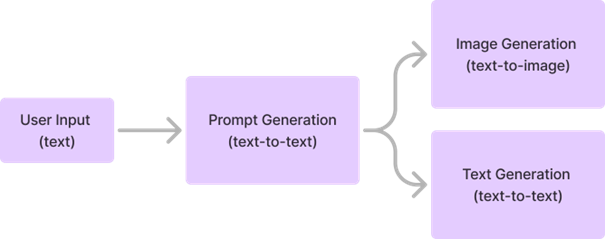
\includegraphics[width=\textwidth]{abbildungen/Process_image_generation}
    \caption{Prozess zur KI gestützten Social Media Content Generierung}
    \label{fig:process_content_generation}
\end{figure}


Der Anwender startet den Prozess mit der Angabe von Informationen über das gewünschte Produkt, für welches der Social Media Content generiert werden soll.
Im ersten Verarbeitungsschritt wird diese Informationen von einem Text-to-Text Machine Learning Modell verarbeitet, um daraus einen prompt zu generieren, welcher als Basis dient, um die finalen Social Media Inhalte zu generieren.
Entscheidend ist hierbei die Erweiterung der Produktangaben um stilistische Anweisungen und werbespezifischen Details, um ein möglichst engagement förderndes Ergebnis zu erzielen.
Der finalisierte Prompt, welcher als Basis für die Generierung von Bild und Text dient, wird anschließend einerseits ein weiteres Mal in ein Text-to-Text Machine Learning Modell übergeben, um daraus eine aussagekräftige Social Media Beschreibung in Textform zu generieren und andererseits in ein Text-to-Image Modell, um ein ansprechendes Bild zu generieren, welches für die Bewerbung des gewünschten Produktes geeignet ist.
Zur Auswahl eines geeigneten Text-to-Image Modelles wurden die beschriebenen Bewertungskriterien herangezogen um eine einheitliche Vergleichsbasis zu schaffen.
Die bewerteten Modelle basieren hierbei auf den populärsten Modellen der Machine Learning Plattform Hugging Faces.

Verglichen wurden unter anderem bekannte Modelle von etablierten Unternehmen wie die stable-diffusion modelle der Firma stability AI oder FLUX Modelle der firma black forest labs.
Um die leistungsfähigkeit der Modelle zu vergleichen und anschließend eine finale Auswahl je Modellziel treffen zu können, wurde ein prompt mit der Anweisung zur Generierung eines Döner Kebabs den verschiedenen Modelle als input übergeben.
Anschließend wurde die benötigte Zeit zur Generierung des outputs, sowie der output selbst miteinander verglichen.

Abbildung \ref{fig:results_image_generation} zeigt eine Zusammenfassung der generierten Inhalte in der Kategorie Text-to-Image.
Positiv zu bewerten ist, dass alle der getesteten Modelle den Auftrag korrekt interpretiert haben und eine Detailaufnahme des geforderten Produktes erzeugt haben.
Unterschiede gibt es jedoch im erreichten Realismus der Produktbilder.
Die FLUX modelle erzeugten hierbei die qualitativ hochwertigsten und realistischsten Bilder, die kaum von realen Produktbildern zu unterscheiden sind.
Die Stable Diffusion Modelle waren ebenfalls dazu fähig, inhaltlich korrekte aber dennoch minderwertige Produktbilder zu generieren.
Bei näherer Betrachtung der abgebildeten Zutaten eine gewisse Künstlichkeit auf, die Rückschlüsse auf KI generierte Inhalte schließen lässt.
Zudem erzeugen die Produktbilder nur mäßiges Interesse am Produkt, aufgrund der vergleichsweisen schlechten Komposition und stilistischen Umsetzung des Bildes.
Das Sana-\_1600M\_1024px Modell erzeugte ein ähnlich gelungenes, visuell ansprechendes Produktbild, wie die Modelle FLUX.1-dev und FLUX.1-schnell, dennoch ist der Realismusgrad deutlich schlechter, da sich die Strukturen der abgebildeten Zutaten leicht von den Originalen unterscheiden.

\begin{figure}[htbp]
    \centering
    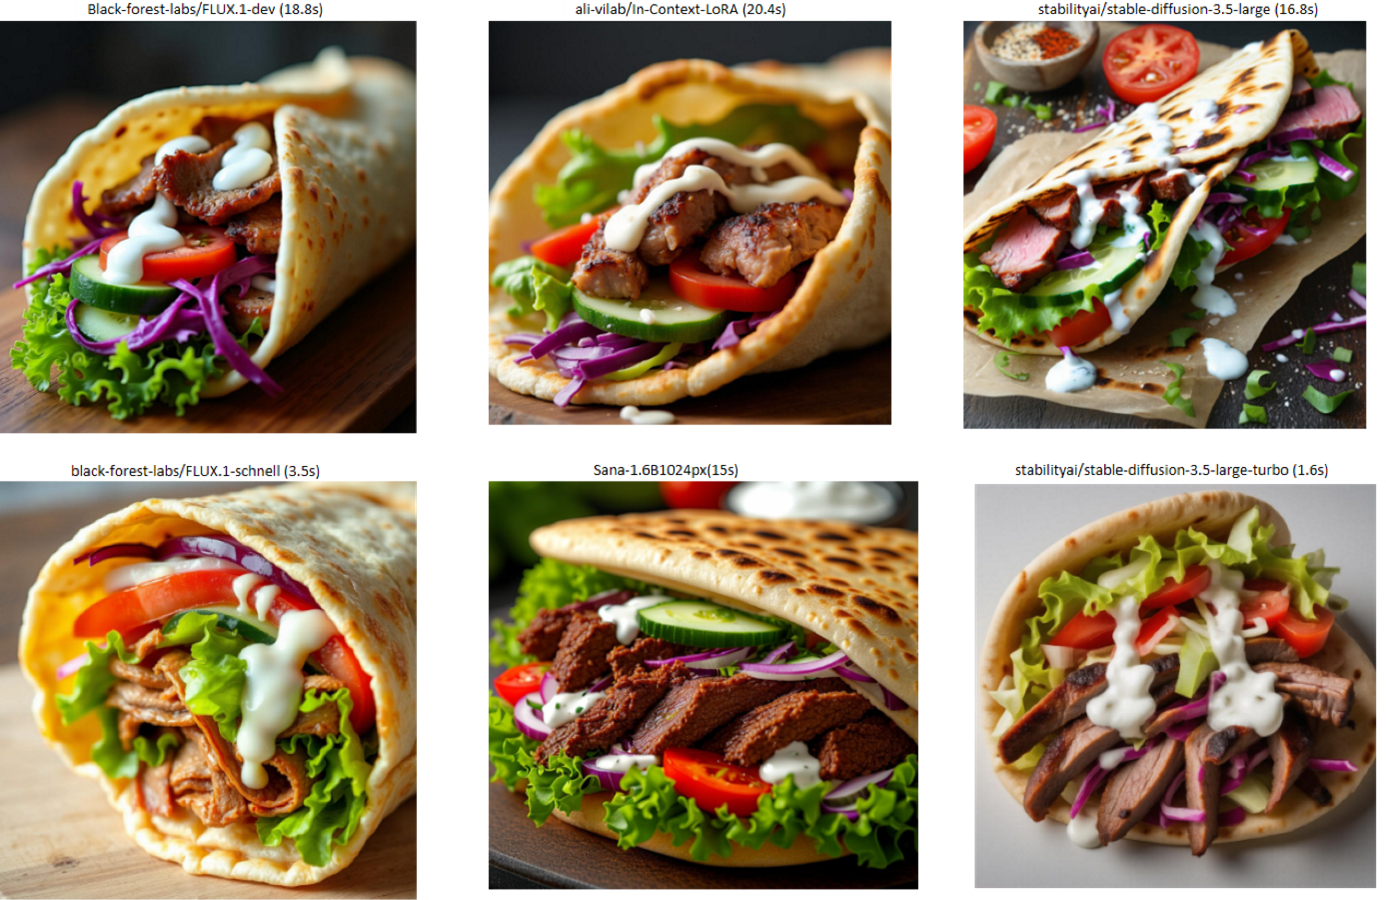
\includegraphics[width=\textwidth]{abbildungen/Results_image_generation}
    \caption{Vergleich der generierten Bilddateien durch die Text-to-Image Modelle}
    \label{fig:results_image_generation}
\end{figure}

Die Abbildungen \ref{fig:textresult_gemini} bis \ref{fig:textresult_nvdia_nemotron} bieten eine Zusammenfassung der generierten Inhalte zum Modellziel Text-to-Text mit den für Werbezwecken einsetzbaren Bildbeschreibungen.
Positiv zu bewerten ist der über alle Modelle hinweg erreichte Realismusgrad.
Jedes der getesteten Modelle erzeugte kurze, aussagekräftige, bildhafte und mit Schlagwörtern gefüllte Texte und baute zudem themenspezifische Hashtags ein.
Keine der generierten Bildbeschreibungen unterscheidet sich stark in Form und Inhalt von heutzutage gängigen Werbebeiträgen in sozialen Medien.
Hierbei auffällig ist, dass sowohl das QwQ-32B-Preview Modell, als auch das Llama-3.1-Nemotron-70B-Instruct-HF standardmäßig keine Emojis als stilistisches Mittel in den generierten Texten verwenden.
Darüber hinaus ist zu beobachten, dass das Llama-3.1-Nemotron-70B-Instruct-HF fiktive Rabattaktionen bewirbt, die nicht im Eingabeprompt gefordert waren.
Alle der untersuchten Text-to-Text Modelle, ausgenommen dem Mistral-7B-Instruct-v0.3 Modell, generierten zudem mehr als eine Bildbeschreibung, obwohl dies nicht im Eingabeprompt verlangt wurde.

\clearpage

\begin{figure}[htbp]
    \centering
    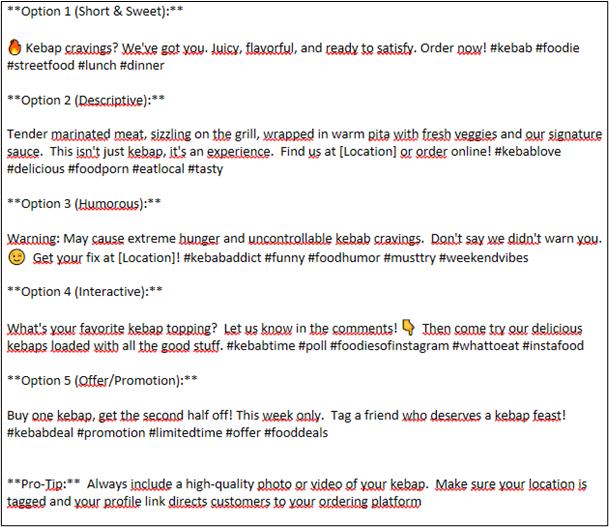
\includegraphics[width=\textwidth]{abbildungen/textresult_gemini}
    \caption{generierter Text durch das Text-to-Text Modell gemini-1.5-pro}
    \label{fig:textresult_gemini}
\end{figure}

\clearpage

\begin{figure}[htbp]
    \centering
    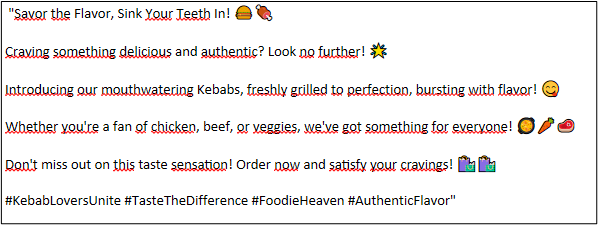
\includegraphics[width=\textwidth]{abbildungen/textresult_mistral}
    \caption{generierter Text durch das Text-to-Text Modell mistralai/Mistral-7B-Instruct-v0.3}
    \label{fig:textresult_mistral}
\end{figure}

\begin{figure}[htbp]
    \centering
    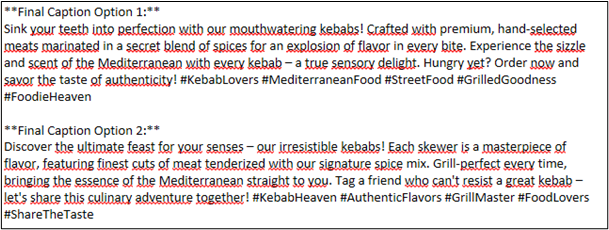
\includegraphics[width=\textwidth]{abbildungen/textresult_Qwen}
    \caption{generierter Text durch das Text-to-Text Modell Qwen/QwQ-32B-Preview}
    \label{fig:textresult_Qwen}
\end{figure}

\clearpage

\begin{figure}[htbp]
    \centering
    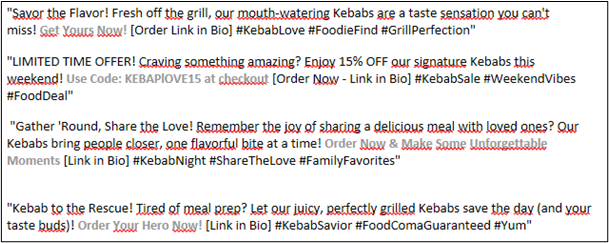
\includegraphics[width=\textwidth]{abbildungen/textresult_nvdia_nemotron}
    \caption{generierter Text durch das Text-to-Text Modell nvidia/Llama-3.1-Nemotron-70B-Instruct-HF}
    \label{fig:textresult_nvdia_nemotron}
\end{figure}

Tabelle \ref{tab:table_modellvergleich} zeigt eine Zusammenfassung der erfassten Kennzahlen über alle untersuchten Modelle.
Auffällig ist jedoch, dass die untersuchten Machine Learning Modelle mit dem Modellziel Text-to-Text, trotz ihrer unterschiedlichen Größe und Trainingsdaten, in der Generierungsdauer und Qualität der Ergebnisse kaum voneinander abweichen.
Die Modellgröße unterscheidet sich jedoch erheblich, wobei das gemini-1.5-pro Modell mit über 100GB das größte Modell, und das Mistral-7B-Instruct-v0.3 mit 15.5GB das kleinste Modell darstellt.
Aus Effizienzgründen ist das Mistral-7B-Instruct-v0.3 Modell für die Kategorie Text-to-Text, welches die qualitativ hochwertigsten Ergebnisse in kürzester Zeit generierte, zu bevorzugen.

Die untersuchten Modelle in der Kategorie Text-to-Image hingegen, zeigen deutliche Unterschiede in der Qualität der generierten Inhalte, wobei die FLUX Modelle die qualitativ hochwertigsten Ergebnisse erzielen.
Im direkten Vergleich erzielte hierbei das FLUX.1-schnell Modell die besten Ergebnisse, da es die qualitativ hochwertigsten Bilder in kürzester Zeit generierte und somit zu bevorzugen ist.

\begin{table}[t]
  \centering
  \begin{tabular}{|p{3cm}|p{3cm}|p{2cm}|p{2cm}|p{3cm}|}
      \hline
      \textbf{Modellname} & \textbf{Modellziel} & \textbf{Modellgröße} & \textbf{Generierungsdauer} & \textbf{Qualität}\\ \hline
      {Black-forest-labs/FLUX.1-dev} & Text-to-Image & 23.8 GB & 18.8s & sehr gut\\ \hline
      {Black-forest-labs/FLUX.1-schnell} & Text-to-Image & 23.8 GB & \textless 5s & sehr gut\\ \hline
      {Efficient-Large-Model/Sana-\_1600M\_1024px} & Text-to-Image & 6.43 GB & \textless 5s & gut\\ \hline
      {Stabilityai/stable-diffusion-3.5-large} & Text-to-Image & 16.5 GB & 16.8s & befriedigend\\ \hline
      {Stabilityai/stable-diffusion-3.5-large-turbo} & Text-to-Image & 16.5 GB & 1.6s & ausreichend\\ \hline
      {Stabilityai/stable-diffusion-3.5-large} & Text-to-Image & 16.5 GB & 1.6s& befriedigend\\ \hline
      {Qwen/QwQ-32B-Preview} & Text-to-Text & \textgreater 50GB & 8s & sehr gut\\ \hline
      {gemini-1.5-pro} & Text-to-Text & \textgreater 100GB & 10s & sehr gut\\ \hline
      {mistralai/Mistral-7B-Instruct-v0.3} & Text-to-Text & 15.5 GB & \textgreater5s & sehr gut\\ \hline
  \end{tabular}
  \caption{Vergleich der generativen Machine Learning Modelle}\label{tab:table_modellvergleich}
\end{table}

\clearpage

\subsection{Auswahlprozess Web-Technologien}
Um geeignete Technologien für die Entwicklung der Applikation zu finden, wird ein Auswahlprozess durchgeführt.

Dieser Prozess folgt dem Konzept der PAPRIKA Methode von Hansen und Ombler.
Zu Beginn wird eine Liste von Kriterien erstellt, die für die Auswahl der Technologien relevant sind.
Anschließend wird eine Gewichtung der Kriterien vorgenommen, um die Relevanz der einzelnen Kriterien zu bestimmen.
Nachdem die Kriterien festgelegt sind, werden die zu vergleichenden Technologien identifiziert.
Abschließend erfolgt die Bewertung der Technologien anhand der Kriterien, indem Diese paarweise miteinander verglichen werden.
Dadurch wird für jede benötigte Komponente die am besten geeignete Technologie identifiziert.\footcite{Paprika2008}

Folgende Anforderungen wurden zur Bewertung der einzelnen Technologien identifiziert:

\begin{table}[htbp]
  \centering
  \begin{tabular}{|p{2cm}|c|p{5cm}|p{4cm}|}
      \hline
      \textbf{Kriterium} & \textbf{Gewicht} & \textbf{Beschreibung} & \textbf{Skala}\\ \hline
      {Lernkurve} & 0.4 & Lernaufwand in Relation zum Erfolgsgrad im Hinblick auf umzusetzende Features & flach, moderat, steil\\ \hline
      {Community} & 0.3 & Größe und Aktivität der Community sowie vorhandenes Lernmaterial & klein, mittel, groß\\ \hline
      {Bibliotheken} & 0.2 & Verfügbarkeit von Bibliotheken & begrenzt, mittel, umfangreich\\ \hline
      {Relevanz} & 0.1 & Aktualität und Weiterentwicklung der Technologie & niedrig, mittel, hoch\\ \hline
  \end{tabular}
  \caption{Bewertung der Anforderungen an Web-Technologien}\label{tab:table}
\end{table}

Im nächsten Schritt werden die zu vergleichenden Technologien identifiziert.
Folgende Komponenten werden für die Entwicklung der Applikation benötigt:

\begin{itemize}
  \item Frontend-Framework
  \item Backend-Framework
  \item Datenbank
\end{itemize}

Um den Auswahlprozess zu vereinfachen, wird die Auswahl auf drei Technologien je Kategorie beschränkt.
Dabei erfolgt die Auswahl anhand von bereits vorhandenem Wissen und Erfahrungswerten.
Es wurden folgende Technologien für die Auswahl identifiziert:

\begin{table}[htbp]
  \centering
  \begin{tabular}{|l|c|c|c|}
      \hline
      \textbf{Technologie Kategorie} & \textbf{Top 1} & \textbf{Top 2} & \textbf{Top 3} \\ \hline
      {Frontend-Framework} & Angular & VueJS & React \\ \hline
      {Backend-Framework} & Flask & Django & Cherrypy \\ \hline
      {Datenbank} & PostgreSQL & MySQL & MongoDB \\ \hline
  \end{tabular}
  \caption{Technologieauswahl Übersicht}\label{tab:Technologieauswahl Übersicht}
\end{table}

Zur Bestimmung der einzelnen Werte werden unterschiedliche Datenquellen herangezogen.
Zur Überprüfung der Relevanz wird die aktuelle Stackoverflow Developer Survey 2024\footcite{StackOverflow2024}, sowie State of JS 2023\footcite{stateofjsStateJavaScript2023} herangezogen.

Zusätzlich werden die Plattformen Github.com und Stackoverflow.com untersucht, inwiefern die Technologien dort vertreten sind.
Für die Frontend Frameworks im Speziellen werden die verfügbaren Libraries im Node Package Manager (NPM) untersucht.

Aus der Analyse lassen sich folgende Daten ableiten:

\begin{table}[h!]
    \centering
    \begin{tabular}{|l|p{2cm}|p{3cm}|p{3cm}|p{3cm}|}
        \hline
        \rowcolor{lightgray} Name & \textbf{Datum Veröffentlichung} & \textbf{Aktive Fragen auf Stackoverflow} & \textbf{Repositories auf Github mit Tag} & \textbf{Abhängigkeiten NPM} \\ \hline
        Angular & 2010\footcite{githubAngularReleaseV090} & 306.845 & 57.588 & 14.607 \\ \hline
        VueJS & 2014\footcite{eggheadEvanYou} & 108.341 & 26.600 & 80.824 \\ \hline
        React & 2013\footcite{githubReactCHANGELOG} & 481.823 & 173.000 & 240.000 \\ \hline
        \hline
        Flask & 2010\footcite{pypiFlask} & 55.856 & 50.985 & - \\ \hline
        Django & 2005\footcite{pypiDjango} & 313.041 & 67.366 & - \\ \hline
        Cherrypy & 2004\footcite{pypiCherryPy} & 1.370 & 147 & - \\ \hline
        \hline
        PostgreSQL & 1996\footcite{postgresqlHappyBirthday} & 178.607 & 56.562 & - \\ \hline
        MySQL & 1995\footcite{amazonWhatMySQL} & 661.661 & 75.826 & - \\ \hline
        Mongodb & 2009\footcite{mongodbMongoDBEvolved} & 176.192 & 111.693 & - \\ \hline
    \end{tabular}
    \caption{Bewertung von Technologien}\label{tab:Analyseergebnise Relevanz der Plattformen}
\end{table}

Darüber hinaus können die Ergebnisse der Studie von Bielek et al. herangezogen werden, welche Aufschluss über die Performance der einzelnen Technologien geben.
Aus der Untersuchung geht hervor, dass VueJS das effizienteste Frontend-Framework ist, gleichzeitig die niedrigste Anzahl an benötigten Programmcodes aufweist.\footcite{Bielak_2022}

Diese Erkenntnisse werden in der Untersuchung von Lipski et al. bestätigt.
Darüber hinaus wird in dieser Studie beschrieben, dass VueJS besonders für Entwickler ohne bisherige Erfahrung in der Webentwicklung geeignet ist.\footcite{Lipski_2021}

Diese Erkenntnisse wirkt sich positiv auf Lernkurve, wie auch die Relevanz der Technologie aus.
Die Syntax von VueJS bricht komplexe Zusammenhänge in einfachere Teile herunter, wodurch die Einarbeitung in die Technologie erleichtert wird.
Dadurch können gleiche Funktionen einfacher und schneller implementiert werden.

Auf Basis der gesammelten Daten und geleisteten Recherchen lassen sich die Technologien wie folgt bewerten:

\begin{table}[h!]
    \centering
    \begin{tabular}{|l|l|c|c|c|c|}
        \hline
        \rowcolor{lightgray} \textbf{Technologie} & \textbf{Kategorie} & \textbf{Community} & \textbf{Lernkurve} & \textbf{Bibliotheken} & \textbf{Relevanz} \\ \hline
        Angular & Backend Framework & \cellcolor{green!70}3 & \cellcolor{red!70}1 & \cellcolor{green!70}3 & \cellcolor{orange!70}2 \\ \hline
        VueJS & Backend Framework & \cellcolor{green!70}3 & \cellcolor{green!70}3 & \cellcolor{orange!70}2 & \cellcolor{green!70}3 \\ \hline
        React & Backend Framework & \cellcolor{green!70}3 & \cellcolor{orange!70}2 & \cellcolor{green!70}3 & \cellcolor{green!70}3 \\ \hline
        Flask & Frontend Framework & \cellcolor{orange!70}2 & \cellcolor{green!70}3 & \cellcolor{orange!70}2 & \cellcolor{orange!70}2 \\ \hline
        Django & Frontend Framework & \cellcolor{green!70}3 & \cellcolor{red!70}1 & \cellcolor{green!70}3 & \cellcolor{green!70}3 \\ \hline
        Cherrypy & Frontend Framework & \cellcolor{red!70}1 & \cellcolor{orange!70}2 & \cellcolor{red!70}1 & \cellcolor{red!70}1 \\ \hline
        PostgreSQL & Datenbank & \cellcolor{green!70}3 & \cellcolor{orange!70}2 & \cellcolor{green!70}3 & \cellcolor{green!70}3 \\ \hline
        MySQL & Datenbank & \cellcolor{green!70}3 & \cellcolor{green!70}3 & \cellcolor{orange!70}2 & \cellcolor{orange!70}2 \\ \hline
        Mongodb & Datenbank & \cellcolor{green!70}3 & \cellcolor{orange!70}2 & \cellcolor{green!70}3 & \cellcolor{green!70}3 \\ \hline
    \end{tabular}
    \caption{Bewertung von Technologien}\label{tab:Tabelle Bewertung von Technologien}
\end{table}

Zuletzt werden die jeweiligen Technologien paarweise miteinander verglichen.
Dabei wird die Bewertung der einzelnen Kriterien in Relation zueinander gesetzt, um die am besten geeignete Technologie zu identifizieren.
Neben den erhobenen Daten fließen auch subjektive Einschätzungen in die Bewertung mit ein.

\textbf{Frontend-Framework:}

Angular und VueJS sind beide als Webtechnologie etabliert und weisen eine entsprechende Community auf.
Ebenso gibt es für beide Tools zahlreiche Communities, wobei sich Angular dort besonders hervortut.
Für die Relevanz der Technologien erscheint VueJS jedoch vielversprechender.
Der entscheidende Faktor in diesem Vergleich ist die Lernkurve der Technologien, bei welcher VueJS mit einer flachen Einstiegserfahrung überzeugt.
Daher fiel die Entscheidung auf VueJS.

Beim Vergleich von Angular und React zeigt sich, dass React ebenfalls äußerst etabliert ist und als eines der beliebtesten Frontend-Frameworks gilt.
Der Umfang an verfügbaren Bibliotheken ist mit Angular vergleichbar.
Jedoch ist die Lernkurve von React im Vergleich zu Angular einfacher, was zu einer Entscheidung zugunsten von React führte.

Der Vergleich von VueJS und React zeigt, dass beide Technologien im Hinblick auf die Community gleichauf sind.
Das Angebot an Bibliotheken ist für React dennoch größer.
Beide Frameworks gelten als äußerst relevant für moderne Applikationen.
Entscheidender Faktor im Vergleich ist die Lernkurve, bei welcher VueJS mit einer flachen Einstiegserfahrung überzeugt.
Aus diesem Grund fiel die Wahl auf VueJS.

In der gesamten Betrachtung der Frontend-Frameworks ist VueJS die Technologie, die am besten zu den Anforderungen passt.

\textbf{Backend-Framework:}

Flask und Django stellen die beiden beliebtesten Python-Frameworks zur Entwicklung von Webapplikationen dar, wobei Django die größere Community aufweist.
Daraus resultiert ein größeres Angebot an Bibliotheken für Django im Vergleich zu Flask.
Ebenso die Relevanz der Technologie ist für Django höher einzustufen.
Über die Lernkurve lässt sich sagen, dass Flask eine flachere Lernkurve aufweist als Django, welches eher als steil zu bewerten ist.
Im direkten Vergleich ist jedoch der Lernaufwand für Django gerechtfertigt, da die Technologie eine Vielzahl an Features bietet und durch die große Community und dem Angebot an Bibliotheken unterstützt wird.
Dadurch ist die Entscheidung auf Django gefallen.

Der Vergleich von Flask und Cherrypy zeigt, dass Flask in allen betrachteten Kriterien besser abschneidet.
Die Community ist größer, das Angebot an Bibliotheken umfangreicher und die Relevanz höher einzustufen.
Auch die Lernkurve wird flacher gewertet als bei Cherrypy, wodurch die Entscheidung, im direkten Vergleich, auf Flask fällt.

Django ist, ebenso wie Flask, in fast allen Kriterien besser zu bewerten als Cherrypy.
Einzig die Lernkurve ist bei Cherrypy flacher einzustufen.
Dennoch überzeugt Django durch die größere Community, das umfangreichere Angebot an Bibliotheken und die höhere Relevanz, weswegen die Entscheidung auf Django fällt.

In der gesamten Betrachtung der Backend-Frameworks ist Django die Technologie, die am besten zu den Anforderungen passt.

\textbf{Datenbanken:}

PostgreSQL und MySQL sind beide als relationale Datenbanken etabliert und weisen eine entsprechende Community auf.
Dabei gilt MySQL als die einsteigerfreundlichere Datenbank während PostgreSQL eine weitere Verbreitung in der gegenwärtigen Technologielandschaft aufweist.
Zudem gilt PostGreSQL als die relevantere Technologie.
Aufgrund der zuvor abgestimmten Gewichtung der Kriterien fällt die Entscheidung auf MySQL.

Der Vergleich von PostgreSQL und MongoDB zeigt, dass die betrachteten Merkmale in etwa gleich zu bewerten sind.
Zentraler Unterschied zwischen beiden Technologien ist die Art der Datenbank, wobei PostgreSQL als relationale Datenbank und MongoDB als NoSQL-Datenbank klassifiziert wird.

Für die Entscheidung über die Datenbanktechnologie wird PostgreSQL als SQL bzw. MongoDB als NoSQL Variante gewählt.
Im Rahmen der Architekturkonzipierung können beide Technologien in Betracht gezogen werden, wobei die Entscheidung auf Basis der spezifischen Anforderungen der Applikation getroffen wird.



